% 2001 年春季上海卷第 19 题：正四棱锥形有盖容器
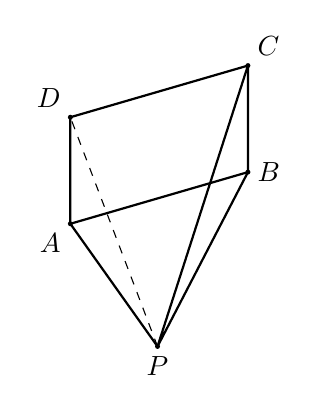
\begin{tikzpicture}[>=stealth, scale=0.82]
  \coordinate (A) at (0,0);
  \coordinate (B) at (2.75,0.8);
  \coordinate (C) at (2.75,2.45);
  \coordinate (D) at (0,1.65);
  \coordinate (P) at (1.35,-1.9);

  \draw[thick] (A)--(B)--(C)--(D)--cycle;
  \draw[thick] (P)--(A) (P)--(B) (P)--(C);
  \draw[dashed] (P)--(D);

  \fill (A) circle (1.1pt) node[below left] {$A$};
  \fill (B) circle (1.1pt) node[right] {$B$};
  \fill (C) circle (1.1pt) node[above right] {$C$};
  \fill (D) circle (1.1pt) node[above left] {$D$};
  \fill (P) circle (1.1pt) node[below] {$P$};
\end{tikzpicture}
